\section{The Model}
\label{sec:model}

\begin{figure*}[!t]
\centering
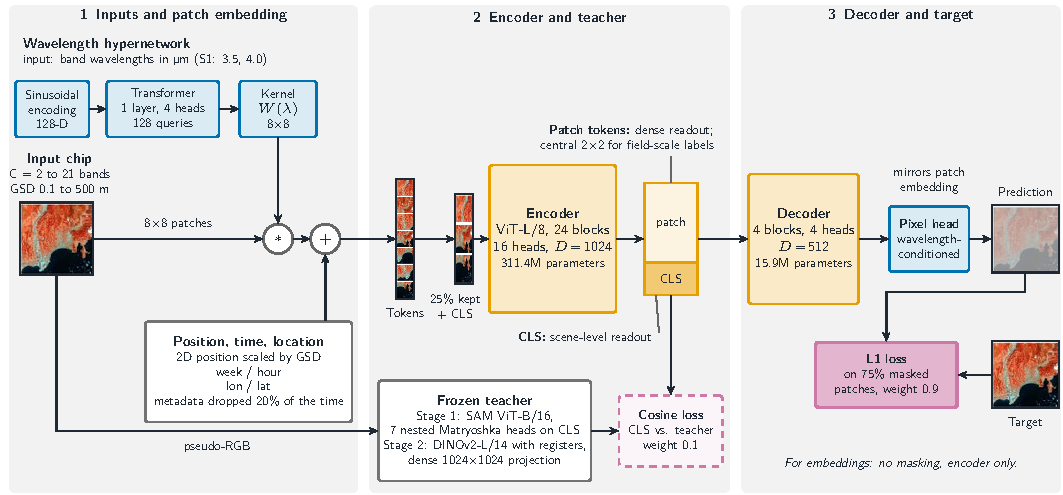
\includegraphics[width=0.95\textwidth]{fig1_architecture_lineage.pdf}
\caption{\textbf{Clay~v1.5 architecture.} (1)~Band wavelengths pass through a hypernetwork (sinusoidal encoding, one transformer layer with 4 heads and 128 queries) that generates the $8\times 8$ patch-embedding kernel, so chips with any band set can be embedded; position, time, and location are added. (2)~A ViT-L/8 encoder ($311.4\text{M}$ parameters) processes the $25\%$ of tokens left unmasked plus a \texttt{CLS} token. \texttt{CLS} is distilled from a frozen teacher (SAM ViT-B/16 in Stage~1, DINOv2-L/14 in Stage~2). (3)~A decoder ($15.9\text{M}$ parameters) reconstructs the masked patches. Loss weights are $0.9$ ($L_1$) and $0.1$ (cosine). Embeddings are computed with the encoder alone.}
\label{fig:arch}
\end{figure*}

Clay~v1.5 was pretrained on $72.1\text{M}$ $256\times 256$ chips ($33.8\,\text{TB}$) across seven open STAC collections spanning $0.5\text{--}500\,\text{m}$ GSD (Table~\ref{tab:corpus}, Figure~\ref{fig:arch}).

\subsection{Pretraining Data}
\label{sec:corpus}

All imagery came from openly licensed public archives. We ingested Sentinel-1 RTC and MODIS MOD09A1 from \textbf{Microsoft Planetary Computer}, which also served the NAIP STAC index. We copied Sentinel-2 L2A (Element~84 Earth Search), NAIP, Landsat~8/9 Collection~2 L1/L2, LINZ, and the $80\,\text{m}$ ESA WorldCover stratification layer from \textbf{AWS Open Data} S3 buckets.

We stratified global scenes from $2{,}728$ unique MGRS tiles ($100\times 100\,\text{km}$, 2018--2023) by $80\,\text{m}$ ESA WorldCover~2021~\cite{zanaga2022worldcover} to oversample human-modified and ecologically diverse landscapes. Built-up, agricultural, and class-diverse strata together account for $77.5\%$ of tile draws; built-up land is drawn at ${\sim}40\times$ its $<1\%$ share of global land. Natural land-cover classes share the remainder. NAIP samples populated places, protected areas, infrastructure, hydrography, and $4{,}000$ random CONUS sites. LINZ samples $50\%$ of New Zealand regional catalogs, and MODIS samples $233$ sinusoidal tiles monthly (2018--2023).

\texttt{stacchip}~\cite{clay2024stacchip} was built to cut $256\times 256$ windows on the fly from Cloud-Optimized GeoTIFFs (COGs) indexed in GeoParquet. But random HTTP/S3 range reads across 2--10 band files per chip left the GPUs waiting on I/O and GDAL decompression. We therefore mirrored selected scenes to S3 and used AWS Batch to pre-pack chips into compressed $128$-chip \texttt{.npz} datacubes per sensor. We split each file into four $32$-chip sub-cubes staged on Amazon FSx for Lustre (\path{/fsx}), so each \texttt{DataLoader} worker reads a contiguous $32$-chip block in a single I/O operation. The train/val split is $80/20$.

\begin{table}[!b]
\centering
\caption{Clay~v1.5 model card and pretraining corpus ($256\times 256$ chips, $33.8\,\text{TB}$; native NAIP $0.6\text{--}1.0\,\text{m}$). Nominal GSD $g$ is passed to the encoder; each $8\times 8$ token covers $8g\times 8g$ ($256g$ chip width). Chip counts are the inventory in the upstream release notes. Training draws equally from the seven collections ($14.3\%$ of steps each), so chips in small collections are drawn more often: a MODIS chip is drawn $7.6$ times as often as it would be if all chips were sampled uniformly ($\times 7.6$), and a NAIP chip half as often ($\times 0.5$).}
\label{tab:corpus}
\scriptsize
\setlength{\tabcolsep}{2.4pt}
\renewcommand{\arraystretch}{0.92}
\begin{tabularx}{\columnwidth}{>{\raggedright\arraybackslash}Xrrrr}
\toprule
\multicolumn{5}{p{0.96\columnwidth}}{\textbf{Clay v1.5} (\texttt{made-with-clay/Clay}~\cite{clay2024hf}) $\cdot$ ViT-L/8 ($311.4\text{M}$ params, $327.3\text{M}$ w/ decoder; vs.\ $95.3\text{M}$ v0, $92.1\text{M}$ v1.0) $\cdot$ Apache-2.0~\cite{clay2024model}} \\
\midrule
Collection (Source) & Bands & GSD & Token & \shortstack[r]{Chips (M)\\ ($\times$ chip share)} \\
\midrule
LINZ Aerial (AWS) & 3 RGB & 0.5\,m & 4\,m & 3.30 ($\times 3.1$) \\
USDA NAIP (PC/AWS) & 4 RGBN & 1.0\,m & 8\,m & 20.98 ($\times 0.5$) \\
Sentinel-2 L2A (AWS) & 10 VSWIR & 10\,m & 80\,m & 18.68 ($\times 0.6$) \\
Sentinel-1 RTC (PC) & 2 SAR & 10\,m & 80\,m & 16.13 ($\times 0.6$) \\
Landsat 8/9 L1 (AWS) & 6 VSWIR & 30\,m & 240\,m & 5.83 ($\times 1.8$) \\
Landsat 8/9 L2 (AWS) & 6 VSWIR & 30\,m & 240\,m & 5.79 ($\times 1.8$) \\
MODIS MOD09A1 (PC) & 7 VSWIR & 500\,m & 4\,km & 1.35 ($\times 7.6$) \\
\midrule
\textbf{Total / Span} & \textbf{2--10} & \textbf{0.5--500\,m} & \textbf{4\,m--4\,km} & \textbf{72.07} \\
\bottomrule
\end{tabularx}
\end{table}

\begin{table*}[!t]
\centering
\caption{Clay~v1.5 against EO and general-purpose models on $43$ benchmarks. \texttt{Best other EO} and \texttt{Best general} give the best EO foundation model other than Clay and the best general-purpose model in each row, with the model tag in brackets. \textbf{\% Best} is Clay divided by the best value in the row, and bold marks that value. A slash separates probe / fine-tuning (Panel B, where the row says so) or \texttt{10-shot / Max} (AlphaEarth/TESSERA rows); each side is bolded on its own and \% Best takes the better ratio. $\pm$ is a $95\%$ bootstrap half-width in Panel~B; in Panel~A it is the leaderboard's reported uncertainty.}
\label{tab:master_bench}
\fontsize{6.5}{7.4}\selectfont
\setlength{\tabcolsep}{1.2pt}
\setlength{\aboverulesep}{0pt}
\setlength{\belowrulesep}{0pt}
\renewcommand{\arraystretch}{0.88}
\newcommand{\slsh}{{/}}
\begin{tabular*}{0.99\textwidth}{@{\extracolsep{\fill}}ll r r l l@{}}
\toprule
Benchmark & Sensor and metric & \textbf{Clay v1.5} & \textbf{\% Best} & Best other EO & Best general \\
\midrule
\multicolumn{6}{@{}l@{}}{\emph{Panel A: SatML leaderboard. Classification, linear probe, 15 core datasets}} \\
\texttt{aid} & Aerial RGB, Acc & 92.8 $\pm$ 1.3 & 94\% & 98.0$^\dagger$ (FarSLIP) & \textbf{98.2} (DINOv3-L, EG2) \\
\texttt{benv2} & Sentinel-1 + 2, micro-mAP & 83.7 $\pm$ 0.6 & 97\% & \textbf{86.4} (Olmo-v1.2-B) & 81.6 (DINOv3-L) \\
\texttt{eurosat} & Sentinel-2, Acc & 98.7 $\pm$ 0.3 & 100\% & \textbf{99.1} (Olmo-v1-B) & 97.9 (ViT-L/16) \\
\texttt{eurosat-spatial} & Sentinel-2, Acc & 96.8 $\pm$ 0.5 & 99\% & \textbf{98.3} (Olmo-v1-L) & 96.1 (ConvNeXt-L) \\
\texttt{forestnet} & Sentinel-2, Acc & 58.3 $\pm$ 3.0 & 98\% & \textbf{59.3} (DEO-B-RGB) & 57.0 (ViT-L/16) \\
\texttt{m-bigearthnet} & Sentinel-2, micro-mAP & 73.1 $\pm$ 1.4 & 93\% & \textbf{78.4} (Olmo-v1.2-B) & 70.9 (DINOv3-L) \\
\texttt{m-brick-kiln} & Sentinel-2, Acc & \textbf{98.0} $\pm$ 0.9 & 100\% & 97.7 (TM-L-RGB) & 97.9 (SwinV2-B) \\
\texttt{m-eurosat} & Sentinel-2, Acc & 96.8 $\pm$ 1.1 & 98\% & \textbf{98.6} (Olmo-v1-L) & 96.4 (DINOv3-L) \\
\texttt{m-forestnet} & Landsat, Acc & 57.5 $\pm$ 3.1 & 98\% & \textbf{58.9} (DEO-B-RGB) & 56.3 (Swin-L) \\
\texttt{m-pv4ger} & Aerial RGB, Acc & 96.1 $\pm$ 1.1 & 98\% & 97.1 (DOFA-L) & \textbf{97.9} (ConvNeXt-L) \\
\texttt{m-so2sat} & Sentinel-1 + 2, Acc & 73.0 $\pm$ 2.7 & 98\% & \textbf{74.4} (Olmo-v1.1-B) & 67.2 (DINOv3-L) \\
\texttt{resisc45} & Aerial RGB, Acc & 88.1 $\pm$ 0.7 & 92\% & 95.2$^\dagger$ (FarSLIP) & \textbf{95.8} (DINOv3-L) \\
\texttt{so2sat} & Sentinel-1 + 2, Acc & 73.0 $\pm$ 2.9 & 98\% & \textbf{74.8} (Olmo-v1-L) & 67.2 (DINOv3-L) \\
\texttt{treesatai} & Aerial + S1/S2, micro-mAP & 63.0 $\pm$ 1.4 & 93\% & \textbf{68.1} (DINOv3-SAT) & 65.8 (DINOv3-L) \\
\texttt{ucmerced} & Aerial RGB, Acc & 96.7 $\pm$ 1.6 & 97\% & \textbf{99.3} (DOFA-L) & 99.0 (EfficientNetV2-L) \\
\multicolumn{6}{@{}l@{}}{\emph{Segmentation, UPerNet head (Clay: our runs in the leaderboard's harness)}} \\
\texttt{sen1floods11-s2} & Sentinel-2, mIoU & 87.0$^\dagger$ & 98\% & \textbf{89.0} (Olmo-v1.2-B) & 78.7 (SwinV2-L) \\
\texttt{sen1floods11-s1} & Sentinel-1, mIoU & 79.0$^\dagger$ & 96\% & \textbf{82.2} (Olmo-v1.2-B) & 81.7 (SwinV2-L) \\
\texttt{burn\_scars} & HLS, mIoU & 86.1$^\dagger$ & 92\% & \textbf{94.0} (Pr.-2) & 90.0 (DINOv3-L) \\
\midrule
\multicolumn{6}{@{}l@{}}{\emph{Panel B: Benchmarks used by peers (our runs). OlmoEarth v1.3, GEO-Bench and Copernicus-Bench tasks, linear probe or fine-tune}} \\
\texttt{m-pv4ger-seg} & Aerial RGB $0.1\,\text{m}$ (mIoU) & \textbf{84.3} & 100\% & 80.0$^\natural$ (Olmo) & 77.9 (DINOv2) \\
\texttt{m-chesapeake} & NAIP RGBN $1.0\,\text{m}$ (mIoU) & \textbf{66.9} & 100\% & 59.9 (Pan.) & 60.2 (DINOv2) \\
\texttt{Biomass-S3}$^\ast$ & S3 OLCI $300\,\text{m}$, 21b ($R^2$) & 0.538 & 91\% & \textbf{0.594}$^\natural$ (Olmo) & 0.451 (DINOv2) \\
\texttt{LC100Cls-S3}$^{\ast\ddagger}$ & S3 OLCI $300\,\text{m}$, 21b (mAP) & 71.6 & 94\% & \textbf{76.4} (Pan.) & 69.1 (DINOv2) \\
\texttt{EuroSAT-S1}$^\ddagger$ & S1 land use (OA) & 85.9 & 97\% & \textbf{88.7} (Pan.) & 84.0 (DINOv2) \\
\texttt{Vessel Detect.\ (S1)} & S1 vessels (FT $F_1$) & 77.5$^\S$ & 97\% & \textbf{79.6} (TM-B) & n/a \\
\texttt{Vessel Detect.\ (L8)} & Landsat-8 vessels (FT $F_1$) & 66.4$^\S$ & 89\% & \textbf{74.9} (Pan.) & n/a \\
\texttt{Solar Farm Detect.} & S2 10b solar (FT mIoU) & 81.8 & 93\% & \textbf{87.5} (Olmo) & 70.7 (DINO) \\
\texttt{MADOS} & S2 debris (LP / FT mIoU) & 52.4 \slsh{} 68.8 & 92\% & \textbf{68.4} \slsh{} \textbf{74.6} (Gal./Olmo) & 59.7 \slsh{} 64.7 (DINO) \\
\texttt{m-cashewplant} & S2 plantations (LP / FT mIoU) & 20.6 \slsh{} 70.7$^\S$ & 87\% & 51.1 \slsh{} \textbf{81.3} (Pr.-2/TM) & \textbf{54.1} \slsh{} 80.6 (DINO) \\
\multicolumn{6}{@{}l@{}}{\emph{AlphaEarth / TESSERA suite, 15 tasks, 10-shot / Max}} \\
\texttt{Africa crop mask} & Cropland mask (B.Acc) & 0.77 \slsh{} 0.87 & 95\% & \textbf{0.82} \slsh{} \textbf{0.92}$^\diamond$ (Olmo) & 0.77 \slsh{} 0.88 (DINOv2) \\
\texttt{ASTER emissivity} & Thermal emissivity ($R^2$) & 0.75 \slsh{} 0.84 & 98\% & \textbf{0.80} \slsh{} \textbf{0.86} (Olmo) & 0.49 \slsh{} 0.64 (DINOv2) \\
\texttt{LCMAP land cover} & CONUS land cover (B.Acc) & 0.67 \slsh{} 0.74 & 91\% & \textbf{0.74} \slsh{} \textbf{0.84}$^\diamond$ (Olmo/AEF) & 0.55 \slsh{} 0.66 (DINOv2) \\
\texttt{LCMAP land use} & CONUS land use (B.Acc) & 0.66 \slsh{} 0.74 & 88\% & \textbf{0.75} \slsh{} \textbf{0.89}$^\diamond$ (Olmo) & 0.54 \slsh{} 0.57 (DINOv2) \\
\texttt{LCMAP cover change} & Cover change (B.Acc) & 0.56 \slsh{} 0.58 & 90\% & \textbf{0.62} \slsh{} \textbf{0.78}$^\diamond$ (AEF) & 0.50 \slsh{} 0.51 (DINOv2) \\
\texttt{LCMAP use change} & Use change (B.Acc) & 0.53 \slsh{} 0.56 & 95\% & \textbf{0.56} \slsh{} \textbf{0.79}$^\diamond$ (TES/AEF) & 0.49 \slsh{} 0.45 (DINOv2) \\
\texttt{Oil palm (Descals)} & Oil palm extent (B.Acc) & 0.65 \slsh{} 0.71 & 86\% & \textbf{0.76} \slsh{} \textbf{0.84} (Olmo) & 0.65 \slsh{} 0.79 (DINOv2) \\
\texttt{GLanCE land cover} & Global land cover (B.Acc) & 0.49 \slsh{} 0.59 & 86\% & \textbf{0.57} \slsh{} \textbf{0.71}$^\diamond$ (Olmo) & 0.38 \slsh{} 0.44 (DINOv2) \\
\texttt{LUCAS land use} & Europe land use (B.Acc) & 0.23 \slsh{} 0.26 & 77\% & \textbf{0.30} \slsh{} \textbf{0.39}$^\diamond$ (Olmo/AEF) & 0.18 \slsh{} 0.20 (DINOv2) \\
\texttt{LUCAS land cover} & Europe land cover (B.Acc) & 0.18 \slsh{} 0.22 & 55\% & \textbf{0.33} \slsh{} \textbf{0.41}$^\diamond$ (TES) & 0.10 \slsh{} 0.12 (DINOv2) \\
\texttt{Canada crops (crs.)} & Coarse crop types (B.Acc) & 0.35 \slsh{} 0.48 & 65\% & \textbf{0.57} \slsh{} \textbf{0.74}$^\diamond$ (Olmo) & 0.24 \slsh{} 0.29 (DINOv2) \\
\texttt{Canada crops (fine)} & Fine crop types (B.Acc) & 0.35 \slsh{} 0.45 & 68\% & \textbf{0.54} \slsh{} \textbf{0.66}$^\diamond$ (Olmo) & 0.17 \slsh{} 0.22 (DINOv2) \\
\texttt{Ethiopia crops} & Smallholder crops (B.Acc) & 0.31 \slsh{} 0.32 & 84\% & \textbf{0.37} \slsh{} \textbf{0.69}$^\diamond$ (TES/AEF) & 0.27 \slsh{} 0.33 (DINOv2) \\
\texttt{US tree genera} & Tree genera, 39c (B.Acc) & 0.07 \slsh{} 0.09 & 54\% & \textbf{0.13} \slsh{} \textbf{0.23}$^\diamond$ (Olmo) & 0.07 \slsh{} 0.07 (DINOv2) \\
\texttt{OpenET monthly ET} & S2 flux ($R^2$) & 0.12 \slsh{} 0.45 & 80\% & \textbf{0.15} \slsh{} \textbf{0.58}$^\diamond$ (Olmo/AEF) & \text{--}0.27 \slsh{} 0.09 (DINOv2) \\
\midrule
\textbf{Median, all panels} & 43 rows & 1 checkpoint & \textbf{94\%} & 11 model families & 7 model families \\
\bottomrule
\end{tabular*}
\par\smallskip
\begin{minipage}{0.99\textwidth}
\scriptsize\setlength{\parskip}{1.5pt}
\textbf{Sources.} Panel~A is read from the SatML leaderboard~\cite{taylorgeospatial2026satml} at harness commit \texttt{83ca5cb} (2026-11-16), with the best band set and normalization per model; Clay's $\pm$ there is the leaderboard's, for one run. In the segmentation rows, Clay is the mean of 3 seeds with a frozen encoder, while leaderboard cells are the best over seeds and adaptation modes. In Panel~B, \texttt{Best other EO} is the maximum over DOFA-L, OlmoEarth~v1.3, the best other peer, TESSERA, and AlphaEarth, and \texttt{Best general} is DINOv2 or DINOv3; the peer cells of \texttt{Vessel Detect.}, \texttt{Solar Farm Detect.}, \texttt{MADOS}, and \texttt{m-cashewplant} are from~\cite{olmoearth2026v13}. The last row gives the median \% Best over all rows and the number of model families behind each comparison column, where versions and sizes of one model count once.\par
\textbf{Marks.} $^\dagger$Our own run in the leaderboard's harness, of a model the leaderboard does not list or of Clay on a task where it has no entry. $^\ast$Sentinel-3 OLCI, a 21-band sensor not seen in pretraining, with zero-decoder, image-only probes; \texttt{Biomass-S3} is at its native $96\,\text{px}$ (chip $R^2{=}0.790$) and \texttt{LC100Cls-S3} reports macro mAP. $^\ddagger$Chips under $224\,\text{px}$ are resized to $224\times 224$ for the linear probe. $^\natural$Cross-sensor transfer: RGB/NIR bands mapped into \texttt{SENTINEL2\_L2A} \texttt{BandSet 0} with \texttt{MaskValue.MISSING}, as in~\cite{olmoearth2026v13}. $^\S$Single seed: \texttt{Vessel Detect.} at $48{,}000$ steps and \texttt{m-cashewplant} at 100 epochs with the better of two learning rates. Validation had leveled off except on \texttt{Vessel Detect.\ (S1)}. A three-seed run of \texttt{Vessel Detect.\ (S1)} at $6{,}000$ steps gives $63.1$. \cite{olmoearth2026v13} reports $79.9$, $70.7$, and $73.9$ for Clay on these three rows. $^\diamond$Published $10\,\text{m}$ 12-month embeddings: \texttt{Ridge} with $\lambda{=}0$ on the 8 tasks shared with~\cite{olmoearth2026v13}, and the remaining \texttt{Max} cells from~\cite{brown2025alphaearth} Fig.~1A and~\cite{feng2026tesserav2} Table~2.\par
\textbf{Panel~B.} \texttt{DINOv2} uses 3 bands on tasks with more than 3 bands and $[\text{VV},\text{VH},(\text{VV}{+}\text{VH})/2]$ on Sentinel-1.\par
\textbf{AlphaEarth/TESSERA rows.} Single-date ViTs use the central $160\,\text{m}$ patch readout (\texttt{Clay}, \texttt{OlmoEarth}, \texttt{Pr.-2}) or a $224\,\text{px}$ pool (\texttt{DOFA-L}, \texttt{DINOv2}), unless marked $^\diamond$. Unmarked \texttt{Max} cells use the labels available on the matched rows. Unmarked \texttt{TESSERA} / \texttt{AEF} cells use $10\,\text{m}$ v1.1~\cite{feng2026tessera} / $320\,\text{m}$ annual rasters; the published \texttt{AEF} \texttt{OpenET} value ($0.58$) is aligned to the label month.\par
\textbf{Model tags.} \texttt{Olmo-v<V>-<S>}: OlmoEarth version V, size S (B base, L large); \texttt{Olmo}: v1.3. \texttt{DOFA-L}: DOFA Large. \texttt{Pr.-2}: Prithvi-EO-2.0 (600M in Panel~A)~\cite{szwarcman2026prithvi2}. \texttt{TM}, \texttt{TM-<S>}: TerraMind v1, size S, with \texttt{-RGB} for RGB-only input~\cite{jakubik2025terramind}; likewise \texttt{DEO-B-RGB}: DEO Swin-B. \texttt{Gal.}: Galileo~\cite{tseng2025galileo}. \texttt{Pan.}: Panopticon. \texttt{TES}: TESSERA. \texttt{AEF}: AlphaEarth. \texttt{DINOv3-L}, \texttt{DINOv3-SAT}: DINOv3 ViT-L/16 and the satellite-pretrained ViT-L/16~\cite{simeoni2025dinov3}. \texttt{DINOv2}: DINOv2-L~\cite{oquab2024dinov2}. \texttt{DINO}: DINOv2 or DINOv3, as reported. \texttt{EG2}: EmbeddingGemma~2~\cite{schechtervera2026embeddinggemma2}, and \texttt{FarSLIP}: FarSLIP ViT-B/16~\cite{li2025farslip}; both are our runs in the same harness on RGB input. Other tags are leaderboard model names.\par
\textbf{Datasets.}~\cite{mayer2022pv4ger,robinson2019chesapeake,buchhorn2020lc100,santoro2024biomasscci,melton2022openet,wang2025fgmae,lee2021brickkiln,zhu2020so2sat,irvin2020forestnet,kerner2024africacrop,kerner2024africacropdata,hulley2015astergedd,brown2020lcmap,pengra2023lcmapref,descals2021oilpalm,descals2024oilpalm,stanimirova2023glance,dandrimont2020lucas,blasch2024ethct2020,garnot2021pastis,jin2021cashew,kikaki2024mados,sumbul2019bigearthnet,sumbul2021bigearthnetmm,bonafilia2020sen1floods11,helber2019eurosat,cheng2017resisc45,yang2010ucmerced}.
\end{minipage}
\end{table*}

\subsection{Architecture}
\label{sec:arch}

Clay~v1.5 is a ViT-Large masked autoencoder~\cite{dosovitskiy2021vit} with $24$ pre-norm transformer blocks ($D=1024$, $16$ heads). Its $8\times 8$ patch stride yields $L = (H/8)(W/8)$ patch tokens: $1{,}024$ tokens per $256\times 256$ chip, $4\times$ the token density of $16\times 16$ ViTs. A 4-block, 4-head decoder ($D_{\mathrm{dec}}=512$) re-adds the position and metadata encodings to the visible and mask tokens and ends in a wavelength-conditioned pixel head that mirrors the patch embedding. Three conditioning modules adapt the backbone across sensors, scales, and observation contexts:
\begin{enumerate}
  \item \textbf{Wavelength hypernetwork (\texttt{Dynamic\-Embedding}).} A standard ViT binds its input channels to a fixed sensor schema and must be retrained whenever a mission adds channels or shifts spectral windows. \texttt{Dynamic\-Embedding}, adapted from DOFA, generates the $8\times 8$ patch-projection kernel $\bm{W}(\bm{\lambda}) \in \mathbb{R}^{1024 \times C \times 8 \times 8}$ and bias $\bm{b}(\bm{\lambda}) \in \mathbb{R}^{1024}$ on the fly from band center wavelengths $\bm{\lambda} = (\lambda_1,\dots,\lambda_C)$ in micrometers ($\mu\text{m}$). It uses a $128\text{-D}$ sinusoidal encoding, a residual MLP, and a $1$-layer, $4$-head transformer over $128$ learnable weight queries. Queries are initialized with standard deviation $0.02$; generated kernels are multiplied by $0.02$. C-band Sentinel-1 $\gamma^0$ in dB uses pseudo-wavelengths $\lambda_{\mathrm{VV}}=3.5\,\mu\text{m}$ and $\lambda_{\mathrm{VH}}=4.0\,\mu\text{m}$. Because $\bm{W}(\lambda)$ varies smoothly across visible, NIR, and SWIR passbands, shifted band centers across Sentinel-2, Landsat~8/9, NAIP, or unseen $21$-band Sentinel-3 OLCI map onto shared spectral filters at run time. On $320$ held-out Sentinel-2 scenes, dropping from $10$ bands to the $6$ Landsat-equivalent bands retains $95.3\%$ Top-1 retrieval ($\cos=0.940$ on $\overline{\bm{Z}}_{\mathrm{patch}}$) and $R^2=0.807$ (vs.\ $0.839$ on $10$ bands). Every input band therefore needs a center wavelength, so Clay is not suited to derived layers such as DEMs or NDVI.
  \item \textbf{GSD-scaled 2D positional encoding.} An $8\times 8$ token spans $4\times 4\,\text{m}$ on $0.5\,\text{m}$ LINZ orthoimagery but $4\times 4\,\text{km}$ on $500\,\text{m}$ MODIS. Following Scale-MAE, channels $0\text{--}1015$ scale 2D token coordinates by nominal GSD $g$, so self-attention allocates receptive fields by physical ground distance rather than by pixel count alone.
  \item \textbf{Time and location encoding.} The same reflectance means different things across seasons, sun angles, and biomes. Channels $1016\text{--}1023$ append $[\sin,\cos]$ encodings of ISO week, UTC hour, and $(\text{lon},\text{lat})$ coordinates (\texttt{1020..1023}).
\end{enumerate}

\subsection{Training, Compute, and License}
\label{sec:lineage}

A custom sampler and collate function cycle round-robin through the seven sensors, one sensor per step on every GPU ($32$ chips per GPU), and repeat chips from smaller collections so each gets $1/7$ of the steps. We chose this over a curriculum that trains on one sensor for long stretches. Because each mini-batch comes from a single sensor, masked pixel reconstruction alone could leave each sensor in its own embedding space. To favor learning of localized Earth patterns, Clay~v1.5 always masks $75\%$ of patch tokens, a ratio we kept from Clay~v0, where reconstructions looked clearly better at it (an informal judgment, not a sweep). So that the encoder still produces embeddings when inputs are missing, training zeroes time and location together for $20\%$ of 32-chip cubes. For the remaining chips it zeroes all bands with probability $0.10$ and half of the bands with probability $0.20$. Users without time or location pass zeros at inference. To give all sensors one shared target while keeping spectral and spatial detail in the patch tokens, it combines unnormalized masked-patch $L_1$ reconstruction ($\div 10$ on MODIS) with a teacher cosine representation loss on \texttt{CLS} in a $90{:}10$ ratio:
{\small
\begin{equation}
\mathcal{L} = 0.9\,\mathcal{L}_{\mathrm{MAE}\text{-}L_1}(\hat{\bm{X}}_{\mathrm{m}}, \bm{X}_{\mathrm{m}}) + 0.1\,\mathcal{L}_{\mathrm{rep}}(\bm{z}_{\mathrm{CLS}}, \bm{t}_{\mathrm{teach}}),
\label{eq:loss}
\end{equation}}%
The frozen teacher receives pseudo-RGB views (VV, VH, and their mean for Sentinel-1), resized to $518\times 518$ in Stage~2. Training used AdamW~\cite{loshchilov2019adamw} in \texttt{bf16}, with cosine annealing and warm restarts~\cite{loshchilov2017sgdr} every $5{,}000$ steps that cycle the learning rate between $5\times 10^{-6}$ and $5\times 10^{-4}$. \textbf{Stage~1} (Aug--Oct 2024, $78$ epochs) distilled \texttt{CLS} toward pooled SAM ViT-B/16~\cite{kirillov2023sam} features through \textbf{7 nested Matryoshka heads} (\texttt{dolls=[16, 32, 64, 128, 256, 768, 1024]})~\cite{kusupati2022matryoshka}, so that prefixes of \texttt{CLS} could be used alone for compact storage and search. We reconstructed the Stage~1 settings from the public code history. \textbf{Stage~2} (Oct--Nov 2024) switched the teacher to DINOv2-L/14 with registers~\cite{darcet2024registers}. It replaced \texttt{MRLLoss} and its Matryoshka heads with a training-time dense \texttt{nn.Linear(1024, 1024)} projection head $\bm{P}$, discarded at inference; we found that $\bm{P}$ stabilized full-$1{,}024\text{-D}$ probes. We selected the Stage~2 checkpoint at epoch~7 by validation loss. Stage~2 kept Stage~1's variance spike but lost its prefix ordering (\S\ref{sec:lesson_mrl}, Lesson~3).

\textbf{Compute, carbon, and Apache-2.0 relicensing.} Pretraining and catalog exports ran on AWS EC2 in \texttt{us-east-2} (Ohio), on 8-GPU L4, A10G, and L40S instances (\texttt{g6/g5/g6e.48xlarge}). Training ran on a Slurm cluster of these EC2 instances, with PyTorch Lightning DDP across the 8-GPU nodes, all reading the shared FSx for Lustre store. The model fit on one GPU at 32 chips per step, so plain data parallelism was enough. From August to November 2024 the account logged $42{,}031$ EC2 node-hours. The account's reported emissions across all services were $33.56\,\text{tCO}_2\text{e}$ location-based and $0.047\,\text{tCO}_2\text{e}$ market-based, from the AWS Customer Carbon Footprint data export (carbon model v1.0.0). EC2 in \texttt{us-east-2} accounts for $30.59\,\text{tCO}_2\text{e}$ of that ($0.040\,\text{tCO}_2\text{e}$ market-based). Market-based figures follow the GHG Protocol market-based method, which accounts for renewable energy Amazon purchases. These totals cover v1.5 pretraining, tests, and embedding-catalog inference together.

In May~2025 the project relicensed all Clay weights from OpenRAIL-M~\cite{contractor2022rail} to \textbf{Apache-2.0} (documentation CC-BY-4.0). The project's stated reasons (Clay-foundation/model issue~349) were less adoption friction than a non-standard license with use-based restrictions and downstream obligations, consistency with the Apache-2.0 code base, and an explicit patent grant, which CC-BY-4.0 does not provide. Custom licenses also leave open questions that standard licenses avoid: where a license bars military or extractive uses, for example, it is unclear whether disaster response by a defense agency or a regulator's monitoring of a mining concession falls under them.
